\section*{Question 4}
\fakesection{4}

This problem compares the window method of filter design, using a Kaiser window, with the optimal Parks-McClellan method. The aim is to design a high pass FIR filter to meet the following specifications:
\begin{multicols}{2}
    \begin{itemize}
        \item Sampling frequency: $f_s=50$ kHz
        \item Cutoff frequency: $f_c=10$ kHz
        \item Pass band start: $f_p=12$ kHz
        \item Pass band attenuation: $A_p=3$ dB
        \item Stop band attenuation: $A_s=80$ dB
    \end{itemize}
\end{multicols}
Cutoff frequency is the midpoint of the transition band. If the half-width is $f_p-f_c=2$ kHz, then the transition width is $\Delta f=4$ kHz.

To use the Kaiser window design method, several quantities must be determined beforehand:
\begin{itemize}
    \item Maximum pass band ripple: $\delta_p = 1 - 10^{-A_p / 20} \approx 0.29205$
    \item Maximum stop band ripple: $\delta_s = 10^{-A_s / 20} \approx 0.0001$
    \item Required attenuation: $A = -20\log_{10}(\min(\delta_p, \delta_s)) \approx 80$ dB
\end{itemize}
Given these quantities, an initial estimate for the filter length can be made:
\begin{align}
    N = \frac{A - 7.95}{14.36(\Delta f / f_s)} \approx 62.72
\end{align}
Therefore, we initially estimate a filter length of 63. We can now formulate a Kaiser window:
\begin{align}
    w(n) = \frac{I_0(\beta(1 - [2n/(N-1)]^2)^{1/2})}{I_0(\beta)}, \quad |n| \leq (N-1)/2
\end{align}
In (4.2), $I_0$ is the Bessel function of the first kind, evaluated numerically\textsuperscript{1}, and $\beta$ is a piecewise function of the required attenuation, $A$:
\begin{align}
    \beta = \begin{cases}
        0, & A \leq 21 \text{ dB} \\
        0.5842(A - 21)^{0.4} + 0.07886(A - 21), & 21 < A < 50 \\
        0.1102(A - 8.7), & A \geq 50
    \end{cases}
\end{align}
Hence, our value of $\beta$ for $A=80$ dB:
\begin{align}
    \beta = 0.1102(80 - 8.7) \approx 7.85726
\end{align}
We now create the ideal frequency response vector, $V$, in a similar manner to Question 3. The number of bins in the pass band is given by:
\begin{align}
    L = \frac{f_s/2 - f_p}{f_s} \cdot N = 16.38
\end{align}
Therefore, we round this down to 16 bins, producing the DFT-symmetric result of Figure \ref{fig:q4_ideal_freqz}.

\newpage

\begin{figure}[ht]
    \centering
    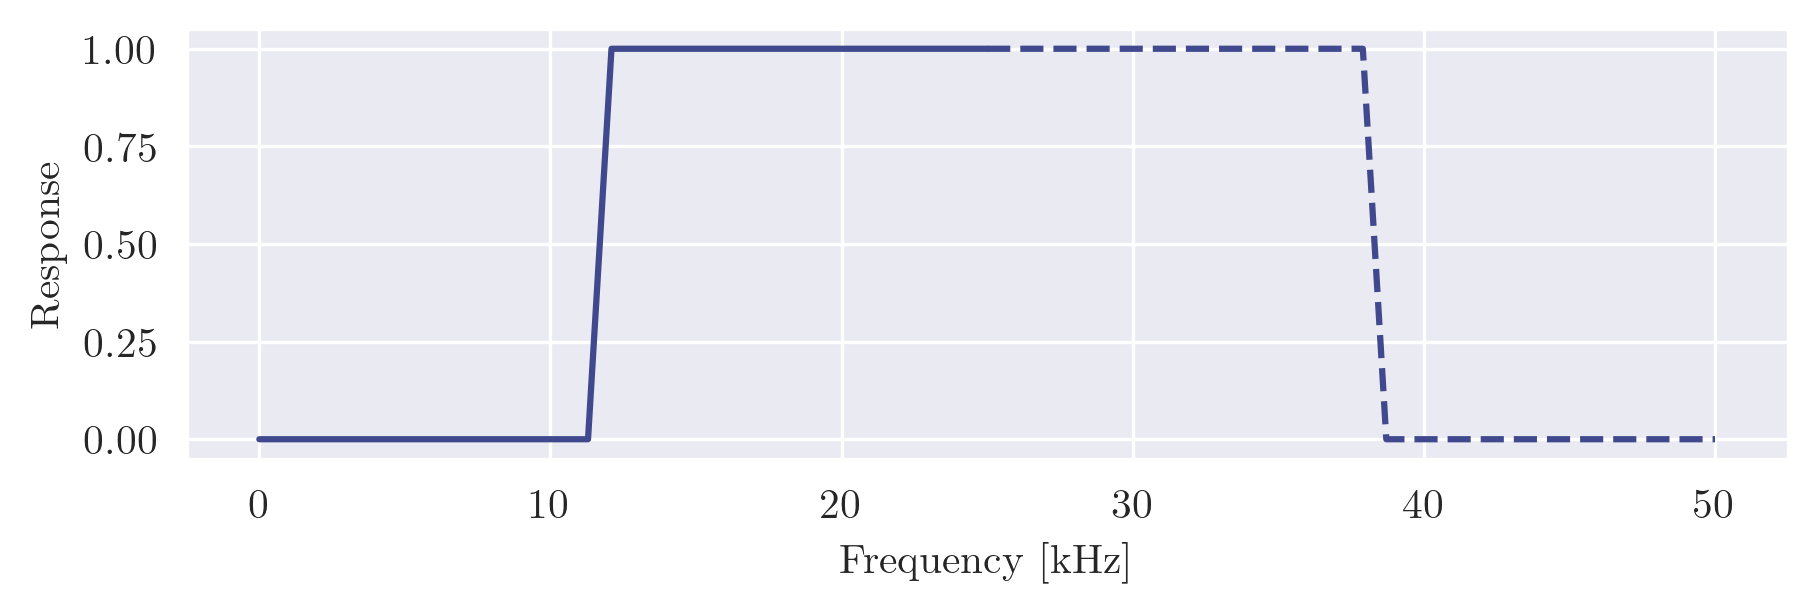
\includegraphics[width=0.8\textwidth]{images/q4_ideal_freqz.png}
    \caption{Frequency response of ideal filter, represented by vector $V$}
    \label{fig:q4_ideal_freqz}
\end{figure}

This has the associated impulse response in the time domain presented in Figure \ref{fig:q4_ideal_impz}.

\begin{figure}[ht]
    \centering
    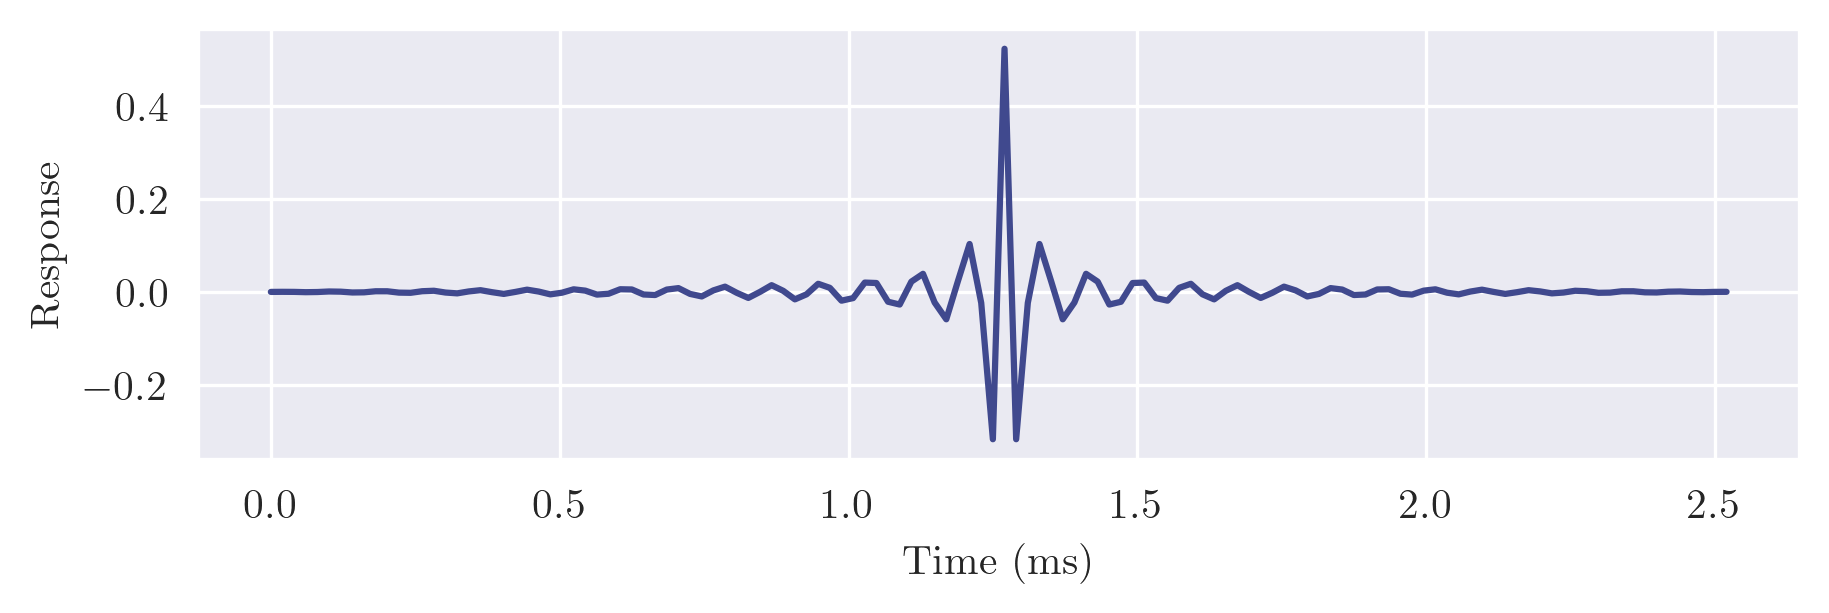
\includegraphics[width=0.8\textwidth]{images/q4_ideal_impz.png}
    \caption{Impulse response of ideal filter}
    \label{fig:q4_ideal_impz}
\end{figure}

We multiply the ideal impulse response by the Kaiser window defined by (4.2) to determine the frequency response of the resulting filter. The results are shown in Figure \ref{fig:q4_kaiser_freqz}.

\begin{figure}[ht]
    \centering
    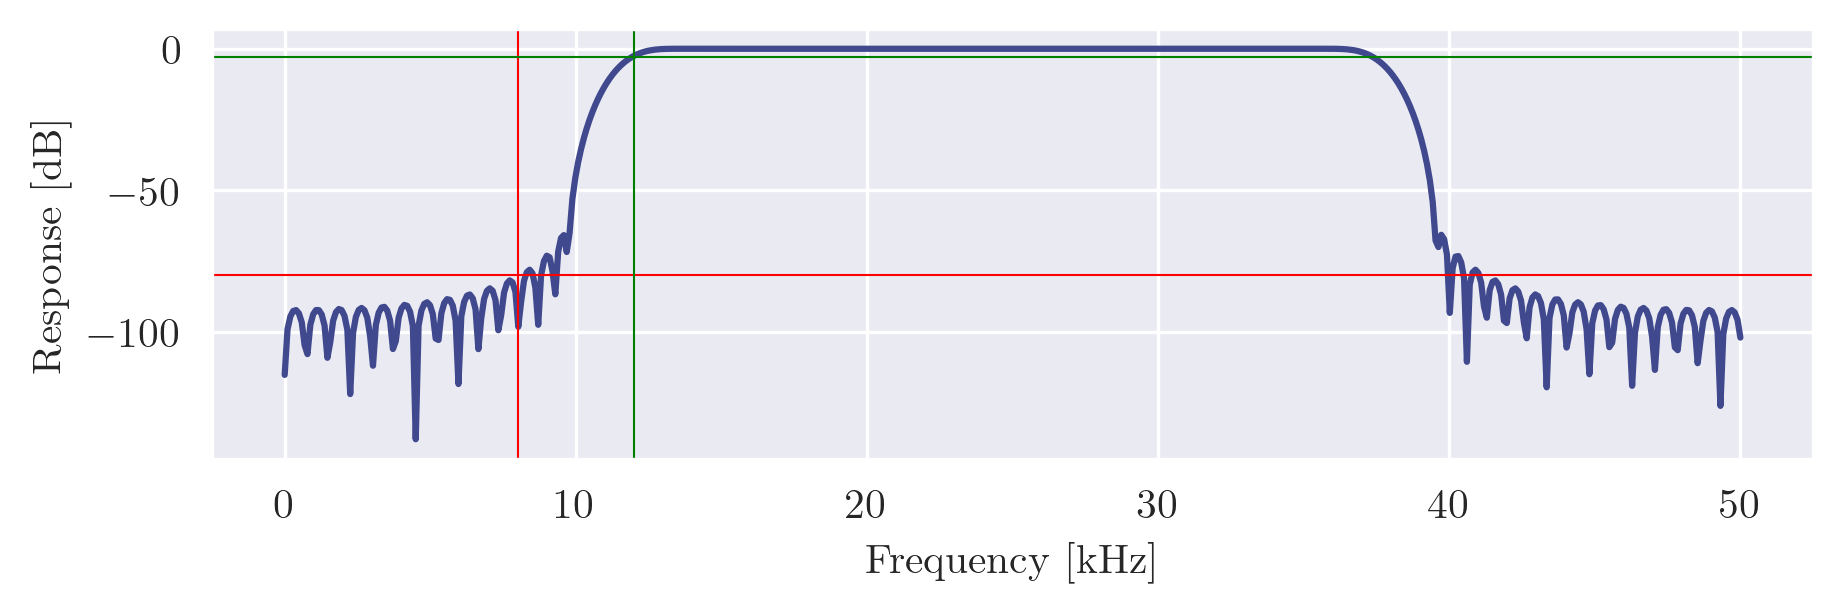
\includegraphics[width=0.8\textwidth]{images/q4_kaiser_freqz.png}
    \caption{Kaiser-windowed filter frequency response; requirements coloured}
    \label{fig:q4_kaiser_freqz}
\end{figure}

Figure \ref{fig:q4_kaiser_freqz} shows that both the stop band (red) and pass band (green) requirements are fulfilled. We now design a filter to the same specifications using the optimal Parks-McClellan method.
